% Options for packages loaded elsewhere
\PassOptionsToPackage{unicode}{hyperref}
\PassOptionsToPackage{hyphens}{url}
%
\documentclass[
]{article}
\usepackage{amsmath,amssymb}
\usepackage{iftex}
\ifPDFTeX
  \usepackage[T1]{fontenc}
  \usepackage[utf8]{inputenc}
  \usepackage{textcomp} % provide euro and other symbols
\else % if luatex or xetex
  \usepackage{unicode-math} % this also loads fontspec
  \defaultfontfeatures{Scale=MatchLowercase}
  \defaultfontfeatures[\rmfamily]{Ligatures=TeX,Scale=1}
\fi
\usepackage{lmodern}
\ifPDFTeX\else
  % xetex/luatex font selection
\fi
% Use upquote if available, for straight quotes in verbatim environments
\IfFileExists{upquote.sty}{\usepackage{upquote}}{}
\IfFileExists{microtype.sty}{% use microtype if available
  \usepackage[]{microtype}
  \UseMicrotypeSet[protrusion]{basicmath} % disable protrusion for tt fonts
}{}
\makeatletter
\@ifundefined{KOMAClassName}{% if non-KOMA class
  \IfFileExists{parskip.sty}{%
    \usepackage{parskip}
  }{% else
    \setlength{\parindent}{0pt}
    \setlength{\parskip}{6pt plus 2pt minus 1pt}}
}{% if KOMA class
  \KOMAoptions{parskip=half}}
\makeatother
\usepackage{xcolor}
\usepackage[margin=1in]{geometry}
\usepackage{color}
\usepackage{fancyvrb}
\newcommand{\VerbBar}{|}
\newcommand{\VERB}{\Verb[commandchars=\\\{\}]}
\DefineVerbatimEnvironment{Highlighting}{Verbatim}{commandchars=\\\{\}}
% Add ',fontsize=\small' for more characters per line
\usepackage{framed}
\definecolor{shadecolor}{RGB}{248,248,248}
\newenvironment{Shaded}{\begin{snugshade}}{\end{snugshade}}
\newcommand{\AlertTok}[1]{\textcolor[rgb]{0.94,0.16,0.16}{#1}}
\newcommand{\AnnotationTok}[1]{\textcolor[rgb]{0.56,0.35,0.01}{\textbf{\textit{#1}}}}
\newcommand{\AttributeTok}[1]{\textcolor[rgb]{0.13,0.29,0.53}{#1}}
\newcommand{\BaseNTok}[1]{\textcolor[rgb]{0.00,0.00,0.81}{#1}}
\newcommand{\BuiltInTok}[1]{#1}
\newcommand{\CharTok}[1]{\textcolor[rgb]{0.31,0.60,0.02}{#1}}
\newcommand{\CommentTok}[1]{\textcolor[rgb]{0.56,0.35,0.01}{\textit{#1}}}
\newcommand{\CommentVarTok}[1]{\textcolor[rgb]{0.56,0.35,0.01}{\textbf{\textit{#1}}}}
\newcommand{\ConstantTok}[1]{\textcolor[rgb]{0.56,0.35,0.01}{#1}}
\newcommand{\ControlFlowTok}[1]{\textcolor[rgb]{0.13,0.29,0.53}{\textbf{#1}}}
\newcommand{\DataTypeTok}[1]{\textcolor[rgb]{0.13,0.29,0.53}{#1}}
\newcommand{\DecValTok}[1]{\textcolor[rgb]{0.00,0.00,0.81}{#1}}
\newcommand{\DocumentationTok}[1]{\textcolor[rgb]{0.56,0.35,0.01}{\textbf{\textit{#1}}}}
\newcommand{\ErrorTok}[1]{\textcolor[rgb]{0.64,0.00,0.00}{\textbf{#1}}}
\newcommand{\ExtensionTok}[1]{#1}
\newcommand{\FloatTok}[1]{\textcolor[rgb]{0.00,0.00,0.81}{#1}}
\newcommand{\FunctionTok}[1]{\textcolor[rgb]{0.13,0.29,0.53}{\textbf{#1}}}
\newcommand{\ImportTok}[1]{#1}
\newcommand{\InformationTok}[1]{\textcolor[rgb]{0.56,0.35,0.01}{\textbf{\textit{#1}}}}
\newcommand{\KeywordTok}[1]{\textcolor[rgb]{0.13,0.29,0.53}{\textbf{#1}}}
\newcommand{\NormalTok}[1]{#1}
\newcommand{\OperatorTok}[1]{\textcolor[rgb]{0.81,0.36,0.00}{\textbf{#1}}}
\newcommand{\OtherTok}[1]{\textcolor[rgb]{0.56,0.35,0.01}{#1}}
\newcommand{\PreprocessorTok}[1]{\textcolor[rgb]{0.56,0.35,0.01}{\textit{#1}}}
\newcommand{\RegionMarkerTok}[1]{#1}
\newcommand{\SpecialCharTok}[1]{\textcolor[rgb]{0.81,0.36,0.00}{\textbf{#1}}}
\newcommand{\SpecialStringTok}[1]{\textcolor[rgb]{0.31,0.60,0.02}{#1}}
\newcommand{\StringTok}[1]{\textcolor[rgb]{0.31,0.60,0.02}{#1}}
\newcommand{\VariableTok}[1]{\textcolor[rgb]{0.00,0.00,0.00}{#1}}
\newcommand{\VerbatimStringTok}[1]{\textcolor[rgb]{0.31,0.60,0.02}{#1}}
\newcommand{\WarningTok}[1]{\textcolor[rgb]{0.56,0.35,0.01}{\textbf{\textit{#1}}}}
\usepackage{graphicx}
\makeatletter
\def\maxwidth{\ifdim\Gin@nat@width>\linewidth\linewidth\else\Gin@nat@width\fi}
\def\maxheight{\ifdim\Gin@nat@height>\textheight\textheight\else\Gin@nat@height\fi}
\makeatother
% Scale images if necessary, so that they will not overflow the page
% margins by default, and it is still possible to overwrite the defaults
% using explicit options in \includegraphics[width, height, ...]{}
\setkeys{Gin}{width=\maxwidth,height=\maxheight,keepaspectratio}
% Set default figure placement to htbp
\makeatletter
\def\fps@figure{htbp}
\makeatother
\setlength{\emergencystretch}{3em} % prevent overfull lines
\providecommand{\tightlist}{%
  \setlength{\itemsep}{0pt}\setlength{\parskip}{0pt}}
\setcounter{secnumdepth}{-\maxdimen} % remove section numbering
\usepackage{longtable}
\usepackage{pdflscape}
\ifLuaTeX
  \usepackage{selnolig}  % disable illegal ligatures
\fi
\usepackage{bookmark}
\IfFileExists{xurl.sty}{\usepackage{xurl}}{} % add URL line breaks if available
\urlstyle{same}
\hypersetup{
  pdftitle={Analysis to Assess the Effects of Two Sets of Reform to a Medical Residents Exam},
  hidelinks,
  pdfcreator={LaTeX via pandoc}}

\title{Analysis to Assess the Effects of Two Sets of Reform to a Medical
Residents Exam}
\author{}
\date{\vspace{-2.5em}}

\begin{document}
\maketitle

\subsection{1 Background}\label{background}

An important standard for medical residents in the US is the internal
medicine certification exam, which serves as a gauge of graduate medical
education efficacy as well as an indicator of individual competency.
Concerns regarding resident workload, exhaustion, and training quality
have led to significant changes in residency programs during the last 20
years. Two particularly significant milestones were the 2003 duty hour
reform, introduced by the Accreditation Council for Graduate Medical
Education (ACGME), and the 2011 revision, which further tightened duty
hour restrictions. While maintaining the caliber of training and board
certification preparation, these reforms sought to strike a balance
between resident well-being and patient safety.

The effect of these reforms on educational outcomes has been a topic of
discussion despite their extensive implementation. Supporters contended
that better-rested residents would learn more efficiently and perform
better on tests, while critics claimed that fewer hours might limit
residents' clinical exposure and jeopardize exam performance. Since the
internal medicine certification exam offers a standardized assessment of
knowledge and preparedness for independent practice, comparing pass
rates over these reform periods provides important information about
whether or not these structural changes were successful.

\subsection{2 Exploratory Data
Analysis}\label{exploratory-data-analysis}

The dataset used in this analysis consists of annual certification exam
results for internal medicine residents across three distinct time
periods: the pre-reform era, the years following the 2003 duty hour
reform, and the years following the 2011 duty hour reform (Appendix 1).

Variables:\\
Year: The year of the exam.\\
N: The number of residents who attempted the exam.\\
Pct: The fraction who passed the exam, expressed as a percentage.

Before proceeding to formal modeling, an exploratory data analysis was
conducted to visualize trends in pass rates, identify patterns across
reform periods, and assess variability in the outcomes.

According to the line plot, the data is divided into three distinct time
periods corresponding to the timing of the reforms (color coded and
labeled in the legend). Pass rates noticeably increased after the first
reform in 2003 compared to the pre-2003 period (Appendix 2). However,
they gradually declined until the second reform in 2011, after which
rates began to rise again. Despite this rebound, the average pass rate
following the 2003 reform (0.91) remained higher than the average after
the 2011 reform (0.86), as shown by the dotted reference lines (Appendix
2).

\subsection{3 Modeling}\label{modeling}

Exam pass rate variability across cohorts was found to be greater than
what could be explained by a standard binomial model, as evidenced by a
residual deviance to degrees-of-freedom ratio of 31.71 (Appendix 7).
This overdispersion implies that there are more underlying variations in
pass probability among cohorts than can be explained by a
straightforward binomial assumption. We chose a beta-binomial model to
address this, which accounts for extra-binomial variability and
appropriately inflates the variance by introducing a dispersion
parameter (\(\rho \approx\) 0.0036). This is the logit of the dispersion
parameter\(\rho\) in the beta-binomial model.

\[
\rho = \frac{\exp(-5.633)}{1 + \exp(-5.633)} \;\approx\; 0.0036
\]

Therefore, the beta-binomial model gives us more realistic confidence
intervals around the estimated pass rates and enables us to model the
inherent heterogeneity among cohorts.

The model's structural division of students into three time periods,
pre-2003, 2003--2010, and post-2011, reflects the training program's
primary reforms and is in line with significant adjustments to the
curriculum, evaluation standards, and policy. This grouping captures
significant changes in pass rates linked to reforms while honoring the
study design and mitigating noise that could result from year-to-year
variations. Future work could include a lag term to account for
potential delayed impacts of reforms on cohorts that underwent multiple
policy changes during their training, even though our current analysis
does not formally include lagged reform effects.

Lastly, the comparison of fitted probabilities and 95\% CI bands with
observed pass rates and their binomial error bars provides evidence for
the validity of the model (Appendix 6). The observed rates show that the
model fits the data better because they are mostly contained within the
beta-binomial intervals but often fall outside the binomial confidence
intervals.

\subsection{4 Analysis}\label{analysis}

We compared a Binomial GLM model and a Beta Binomial Regression model to
see which one would best fit our data. For both models, the time periods
(pre-2003, 2003--2010, 2011+) based on when the reforms occurred were
used as the predictor. The residual deviance and pearson chi-square
tests for the Binomial model show the lack of fit due to overdispersion.
The pearson chi-square statistic (545.25 on 17 df) and residual deviance
(539.15 on 17 df) are both larger than their observed values (Appendix
3). The p-values are also very small, which rejects the null hypothesis
of the binomial model being a good fit for the data.~

For the beta binomial model, the residuals plot shows that the points
are randomly scattered around the zero line with no discernable pattern
(Appendix 5). This shows that the beta binomial model captures a
reasonable fit to the data. Furthermore, AIC values were calculated to
evaluate the goodness of fit. The AIC for the beta binomial model
(262.6) was smaller than that of the binomial model (714.1), which shows
that the beta-binomial provided a better fit for the given data
(Appendix 3).

P-values were also calculated for each of the two reform periods to see
whether they improved the exam pass rates. The 2003 reform was
associated with a statistically significant improvement in pass rates
compared to the pre-2003 baseline (p ≈ 2.16e-08, which is \textless{}
0.05) (Appendix 3). The 2011 reform did not show a statistically
significant change in pass rates because the p-value (p ≈ 0.46) was not
less than the alpha level of 0.05. Overall, the results showed that the
2003 reform did indicate an increase in pass rates, the 2011 reform had
no measurable effect, and the beta-binomial model best fit the data that
was provided.

\subsection{5 Conclusion \& Future Work}\label{conclusion-future-work}

Some shortcomings of our analysis came from the limitations of the
dataset, which only provided the pass rate per year overall and did not
show any individual-level variation, such as demographics, residency
rotation, and program resources, limiting control for confounding. A
potential for improvement would come from obtaining program or
resident-level data.

Additionally, our model, which splits the time periods distinctly into
three groups, assumes immediate changes and jumps instantly to a new
level the moment a reform starts, rather than the possibility of
phasing-in effects, which is more realistic as residents are trained
across three academic years and gradually would increase exposure to the
reform effects. In the future, it could be possible to use interrupted
time series to analyze outcomes measured over time, using the pre-2003
years as the baseline and estimating the jump and new slope after the
2003 and 2011 reforms.

Using a beta-binomial model with the reform periods (pre-2003,
2003-2010, 2011 onward), we find strong evidence that the reform
implemented in 2003 is related to a statistically significant increase
in the medical certification exam pass rates in a year compared to
pre-2003 (p-value \textless\textless{} 0.05), while the reform
implemented in 2011 shows no statistically significant change compared
to pre-2003 and has lower average rates than 2003-2010. The
beta-binomial model was favored compared to the binomial due to its
lower AIC, and the residuals show no systematic pattern. These
conclusions are consistent with prior evidence in medical education,
where it is likely that the 80-hour cap on duty hours implemented in
2003 likely improved rest and study time, supporting higher pass rates,
while the cap on first-year resident shift times introduced 2011 reduced
clinical exposure.

\subsection{6 Appendix}\label{appendix}

\begin{enumerate}
\def\labelenumi{\arabic{enumi}.}
\tightlist
\item
  Table Output
\end{enumerate}

\begin{verbatim}
##   Year    N  Pct
## 1 1996 6964 0.82
## 2 1997 7173 0.85
## 3 1998 7348 0.84
## 4 1999 7311 0.85
## 5 2000 7048 0.86
## 6 2001 6802 0.88
\end{verbatim}

\begin{enumerate}
\def\labelenumi{\arabic{enumi}.}
\setcounter{enumi}{1}
\tightlist
\item
  EDA Graph and Average
\end{enumerate}

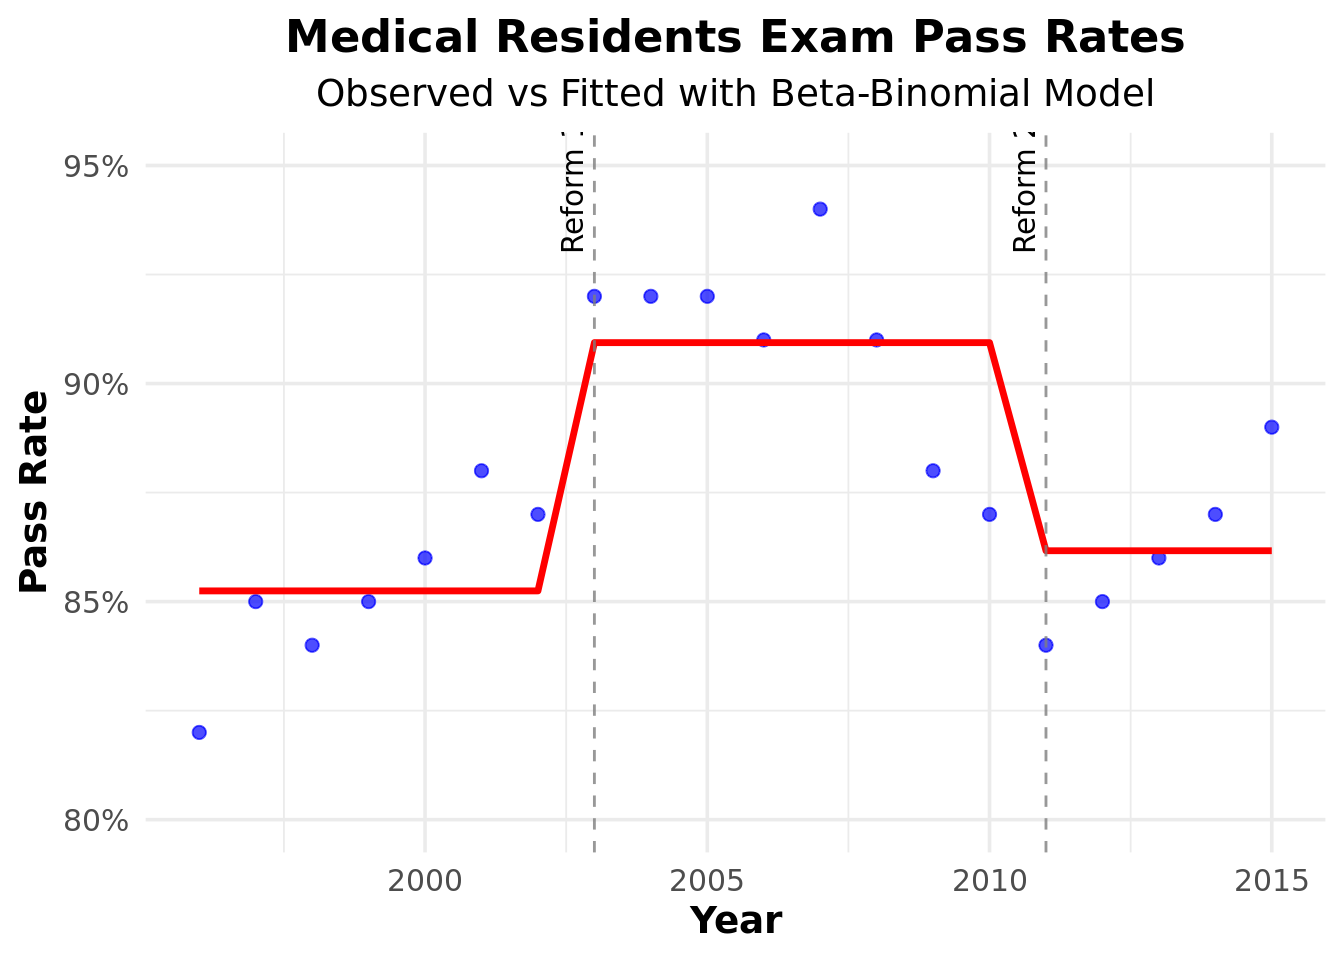
\includegraphics{FinalReport_files/figure-latex/unnamed-chunk-3-1.pdf}

\begin{verbatim}
##                       Period       Pct
## 1   Pre-2003 (before reform) 0.8528571
## 2 2003-2010 (after reform 1) 0.9087500
## 3     2011+ (after reform 2) 0.8620000
\end{verbatim}

\begin{enumerate}
\def\labelenumi{\arabic{enumi}.}
\setcounter{enumi}{2}
\tightlist
\item
  Beta-Binomial Summary Table
\end{enumerate}

\begin{verbatim}
##                     Predictor Log_Odds Std_Error Z_value   P_value Odds_Ratio
## (Intercept):1  (Intercept) mu    1.754     0.065  27.100 9.76e-162      5.778
## timeperiodtp2   timeperiodtp2    0.552     0.099   5.599  2.16e-08      1.737
## timeperiodtp3   timeperiodtp3    0.075     0.102   0.740  4.59e-01      1.078
## (Intercept):2 (Intercept) rho   -5.633     0.329 -17.140  7.50e-66         NA
##               CI_lower CI_upper Predicted_Prob
## (Intercept):1    5.089    6.559          0.852
## timeperiodtp2    1.432    2.107          0.635
## timeperiodtp3    0.883    1.316          0.519
## (Intercept):2       NA       NA             NA
\end{verbatim}

\begin{enumerate}
\def\labelenumi{\arabic{enumi}.}
\setcounter{enumi}{3}
\tightlist
\item
  Beta-Binomial Analysis Table
\end{enumerate}

\begin{verbatim}
## # A tibble: 4 x 2
##   Statistic           Value
##   <chr>               <dbl>
## 1 Pearson Chi-square  545. 
## 2 Residual Deviance   539. 
## 3 Residual df          17  
## 4 Dispersion estimate  31.7
\end{verbatim}

\begin{verbatim}
## # A tibble: 2 x 2
##   Model           AIC
##   <chr>         <dbl>
## 1 Binomial       714.
## 2 Beta-binomial  263.
\end{verbatim}

\begin{enumerate}
\def\labelenumi{\arabic{enumi}.}
\setcounter{enumi}{4}
\tightlist
\item
  Residual Plot
\end{enumerate}

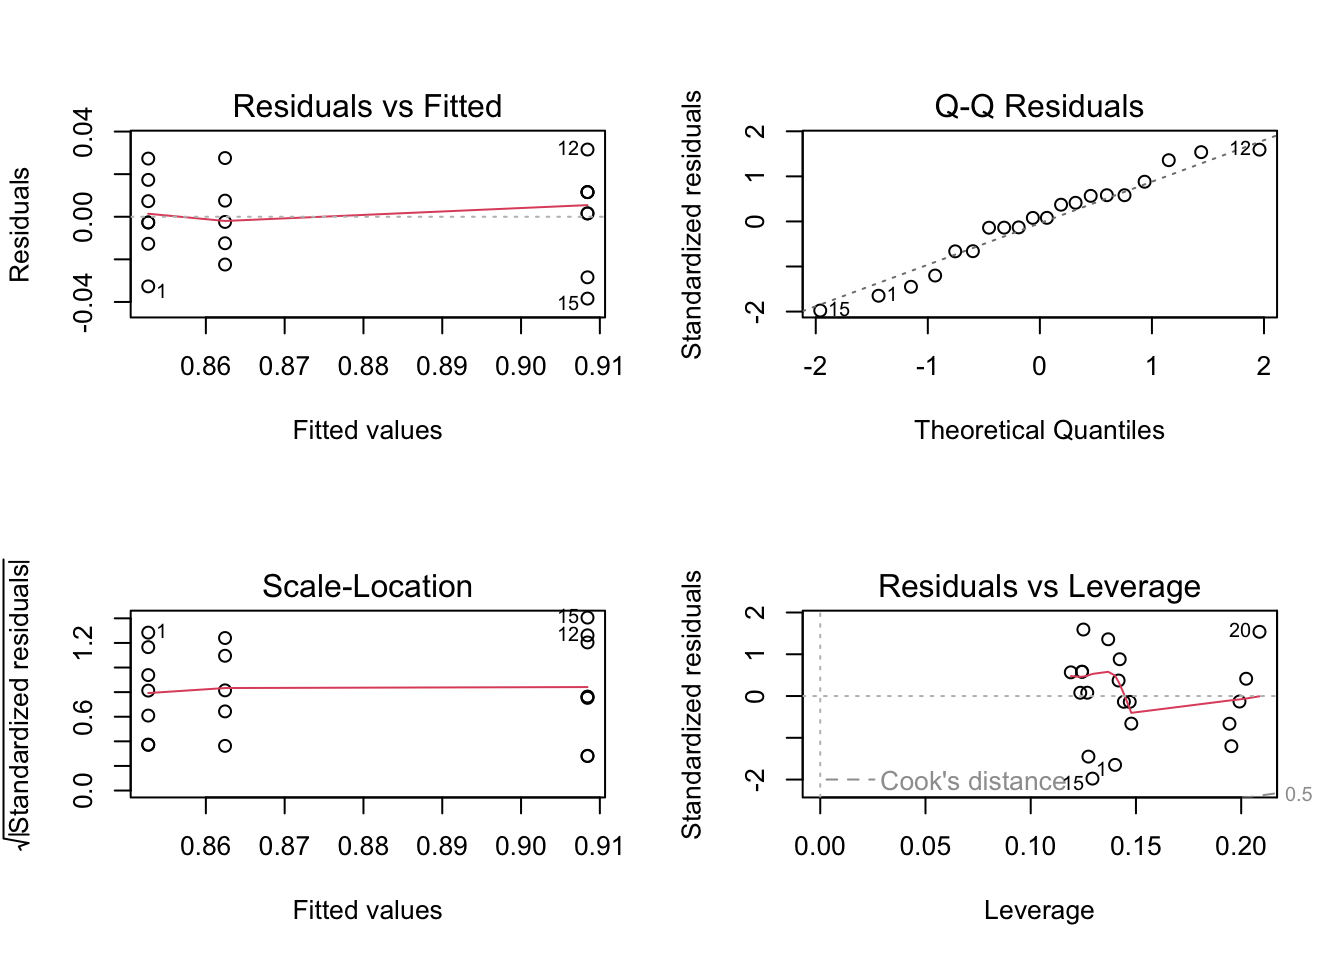
\includegraphics{FinalReport_files/figure-latex/unnamed-chunk-6-1.pdf}

\begin{enumerate}
\def\labelenumi{\arabic{enumi}.}
\setcounter{enumi}{5}
\tightlist
\item
  Beta-Binomial Model Fit
\end{enumerate}

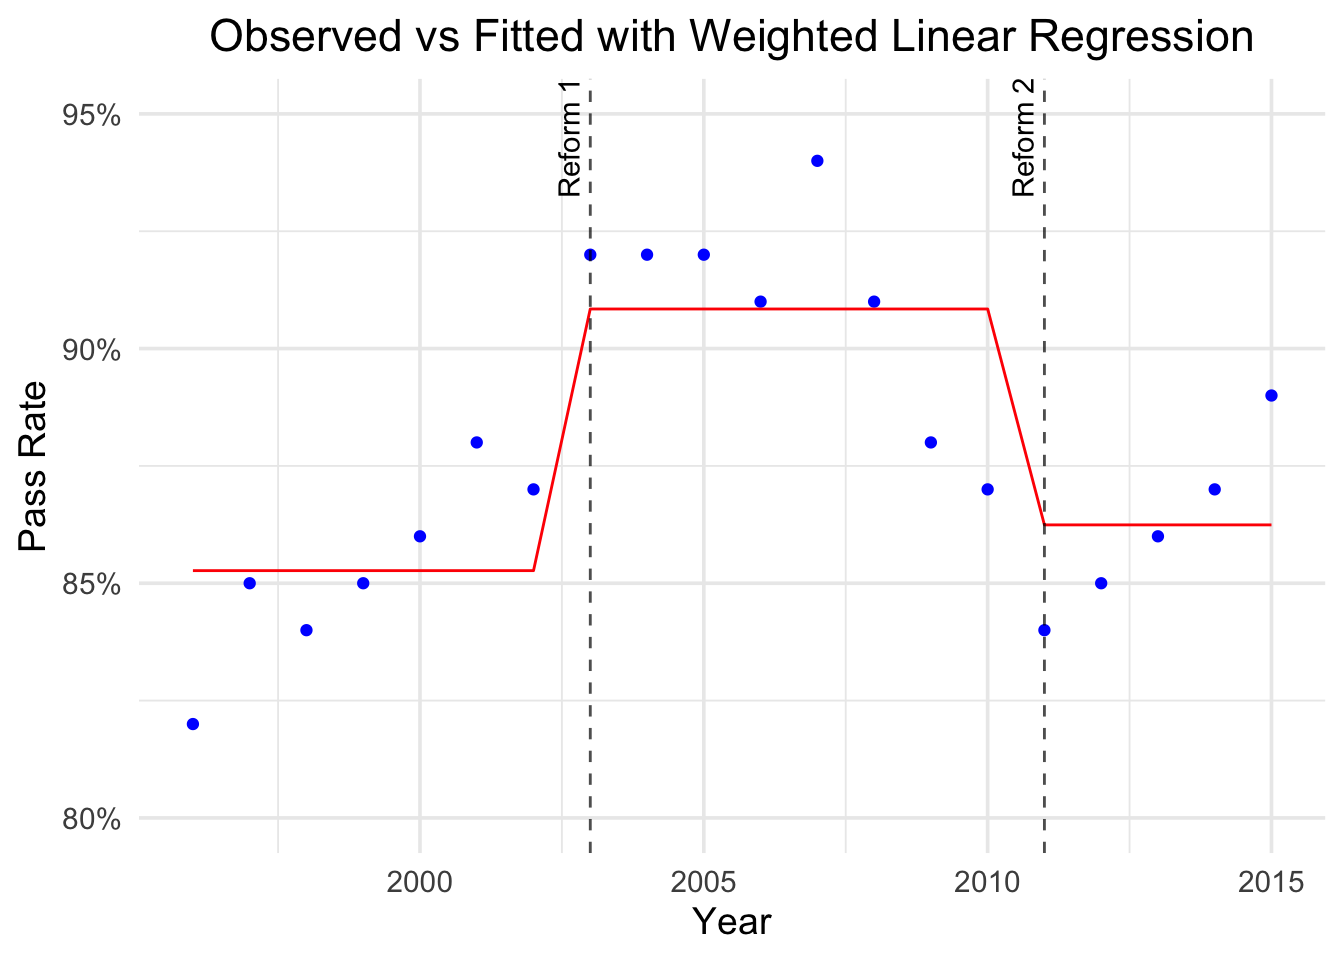
\includegraphics{FinalReport_files/figure-latex/unnamed-chunk-7-1.pdf}

\begin{enumerate}
\def\labelenumi{\arabic{enumi}.}
\setcounter{enumi}{6}
\tightlist
\item
  Binomial Model Dispersion Number
\end{enumerate}

\begin{Shaded}
\begin{Highlighting}[]
\NormalTok{binomial\_model }\OtherTok{\textless{}{-}} \FunctionTok{glm}\NormalTok{(}\FunctionTok{cbind}\NormalTok{(Pass, Fail) }\SpecialCharTok{\textasciitilde{}}\NormalTok{ timeperiod, }
                      \AttributeTok{family =}\NormalTok{ binomial, }\AttributeTok{data =}\NormalTok{ x)}
\NormalTok{res\_dev }\OtherTok{\textless{}{-}} \FunctionTok{deviance}\NormalTok{(binomial\_model)}
\NormalTok{df\_res  }\OtherTok{\textless{}{-}} \FunctionTok{df.residual}\NormalTok{(binomial\_model)}

\NormalTok{dispersion\_ratio }\OtherTok{\textless{}{-}}\NormalTok{ res\_dev }\SpecialCharTok{/}\NormalTok{ df\_res}
\NormalTok{dispersion\_ratio}
\end{Highlighting}
\end{Shaded}

\begin{verbatim}
## [1] 31.71473
\end{verbatim}

Extra:

\begin{Shaded}
\begin{Highlighting}[]
\FunctionTok{library}\NormalTok{(VGAM)}
\FunctionTok{library}\NormalTok{(dplyr)}
\FunctionTok{library}\NormalTok{(broom)}

\CommentTok{\# Fit models}
\NormalTok{binomial\_model }\OtherTok{\textless{}{-}} \FunctionTok{glm}\NormalTok{(}\FunctionTok{cbind}\NormalTok{(Pass, Fail) }\SpecialCharTok{\textasciitilde{}}\NormalTok{ timeperiod, }\AttributeTok{family =}\NormalTok{ binomial, }
                      \AttributeTok{data =}\NormalTok{ x)}
\NormalTok{bb\_model }\OtherTok{\textless{}{-}} \FunctionTok{vglm}\NormalTok{(}\FunctionTok{cbind}\NormalTok{(Pass, Fail) }\SpecialCharTok{\textasciitilde{}}\NormalTok{ timeperiod, betabinomial, }\AttributeTok{data =}\NormalTok{ x)}

\CommentTok{\# Model comparison (AIC)}
\NormalTok{aic\_table }\OtherTok{\textless{}{-}} \FunctionTok{data.frame}\NormalTok{(}
  \AttributeTok{Model =} \FunctionTok{c}\NormalTok{(}\StringTok{"Binomial"}\NormalTok{, }\StringTok{"Beta{-}binomial"}\NormalTok{),}
  \AttributeTok{AIC   =} \FunctionTok{c}\NormalTok{(}\FunctionTok{AIC}\NormalTok{(binomial\_model), }\FunctionTok{AIC}\NormalTok{(bb\_model))}
\NormalTok{)}

\CommentTok{\# Dispersion parameter from beta{-}binomial}
\NormalTok{coef\_all }\OtherTok{\textless{}{-}} \FunctionTok{Coef}\NormalTok{(bb\_model)}
\NormalTok{dispersion\_param }\OtherTok{\textless{}{-}}\NormalTok{ coef\_all[}\StringTok{"(Intercept):2"}\NormalTok{]}

\CommentTok{\# Predicted probabilities with CIs}
\NormalTok{newdat }\OtherTok{\textless{}{-}} \FunctionTok{data.frame}\NormalTok{(}\AttributeTok{timeperiod =} \FunctionTok{factor}\NormalTok{(}\FunctionTok{c}\NormalTok{(}\StringTok{"tp1"}\NormalTok{,}\StringTok{"tp2"}\NormalTok{,}\StringTok{"tp3"}\NormalTok{),}
                                         \AttributeTok{levels =} \FunctionTok{levels}\NormalTok{(x}\SpecialCharTok{$}\NormalTok{timeperiod)))}

\NormalTok{pred\_link }\OtherTok{\textless{}{-}} \FunctionTok{predict}\NormalTok{(bb\_model, }\AttributeTok{newdata =}\NormalTok{ newdat, }\AttributeTok{type =} \StringTok{"link"}\NormalTok{, }\AttributeTok{se.fit =} \ConstantTok{TRUE}\NormalTok{)}
\NormalTok{pred\_prob }\OtherTok{\textless{}{-}} \FunctionTok{plogis}\NormalTok{(pred\_link}\SpecialCharTok{$}\NormalTok{fit)}
\NormalTok{ci\_lower  }\OtherTok{\textless{}{-}} \FunctionTok{plogis}\NormalTok{(pred\_link}\SpecialCharTok{$}\NormalTok{fit }\SpecialCharTok{{-}} \FloatTok{1.96} \SpecialCharTok{*}\NormalTok{ pred\_link}\SpecialCharTok{$}\NormalTok{se.fit)}
\NormalTok{ci\_upper  }\OtherTok{\textless{}{-}} \FunctionTok{plogis}\NormalTok{(pred\_link}\SpecialCharTok{$}\NormalTok{fit }\SpecialCharTok{+} \FloatTok{1.96} \SpecialCharTok{*}\NormalTok{ pred\_link}\SpecialCharTok{$}\NormalTok{se.fit)}

\NormalTok{pred\_table }\OtherTok{\textless{}{-}} \FunctionTok{data.frame}\NormalTok{(}
  \AttributeTok{Period =}\NormalTok{ newdat}\SpecialCharTok{$}\NormalTok{timeperiod,}
  \AttributeTok{Pred\_Prob =} \FunctionTok{round}\NormalTok{(pred\_prob, }\DecValTok{3}\NormalTok{),}
  \AttributeTok{CI\_lower  =} \FunctionTok{round}\NormalTok{(ci\_lower, }\DecValTok{3}\NormalTok{),}
  \AttributeTok{CI\_upper  =} \FunctionTok{round}\NormalTok{(ci\_upper, }\DecValTok{3}\NormalTok{)}
\NormalTok{)}

\CommentTok{\#Combine summary results}
\FunctionTok{list}\NormalTok{(}
  \AttributeTok{AICs =}\NormalTok{ aic\_table,}
  \AttributeTok{Dispersion =}\NormalTok{ dispersion\_param,}
  \AttributeTok{Predictions =}\NormalTok{ pred\_table}
\NormalTok{)}
\end{Highlighting}
\end{Shaded}

\begin{verbatim}
## $AICs
##           Model      AIC
## 1      Binomial 714.1285
## 2 Beta-binomial 262.6229
## 
## $Dispersion
## (Intercept):2 
##      -5.63329 
## 
## $Predictions
##   Period Pred_Prob.logitlink.mu. Pred_Prob.logitlink.rho.
## 1    tp1                   0.852                    0.004
## 2    tp2                   0.909                    0.004
## 3    tp3                   0.862                    0.004
##   CI_lower.logitlink.mu. CI_lower.logitlink.rho. CI_upper.logitlink.mu.
## 1                  0.836                   0.002                  0.868
## 2                  0.897                   0.002                  0.921
## 3                  0.842                   0.002                  0.879
##   CI_upper.logitlink.rho.
## 1                   0.007
## 2                   0.007
## 3                   0.007
\end{verbatim}

\begin{Shaded}
\begin{Highlighting}[]
\CommentTok{\# Extract dispersion coefficient (logit scale)}
\NormalTok{disp\_coef }\OtherTok{\textless{}{-}} \FunctionTok{Coef}\NormalTok{(bb\_model)[}\StringTok{"(Intercept):2"}\NormalTok{]}

\CommentTok{\# Back{-}transform from logit to get rho (dispersion parameter)}
\NormalTok{disp\_param }\OtherTok{\textless{}{-}} \FunctionTok{plogis}\NormalTok{(disp\_coef)}

\FunctionTok{cat}\NormalTok{(}\StringTok{"Dispersion coefficient (logit scale):"}\NormalTok{, disp\_coef, }\StringTok{"}\SpecialCharTok{\textbackslash{}n}\StringTok{"}\NormalTok{)}
\end{Highlighting}
\end{Shaded}

\begin{verbatim}
## Dispersion coefficient (logit scale): -5.63329
\end{verbatim}

\begin{Shaded}
\begin{Highlighting}[]
\FunctionTok{cat}\NormalTok{(}\StringTok{"Estimated dispersion parameter (rho):"}\NormalTok{, disp\_param, }\StringTok{"}\SpecialCharTok{\textbackslash{}n}\StringTok{"}\NormalTok{)}
\end{Highlighting}
\end{Shaded}

\begin{verbatim}
## Estimated dispersion parameter (rho): 0.00356404
\end{verbatim}

The baseline log-odds of passing during the pre-reform era (tp1) are
represented by the intercept for mu. While the coefficient for
timeperiodtp3 shows a smaller increase that is not statistically
significant at conventional levels, the coefficient for timeperiodtp2
shows a statistically significant increase in pass rates in comparison
to the baseline. There is only slight overdispersion in the data, as
indicated by the dispersion parameter (rho), which is small and not
statistically significant.\\
\strut \\
With an AIC of 262.62, the beta-binomial model significantly
outperformed the standard binomial model, which had an AIC of 714.13.
This demonstrates that the beta-binomial model fits data much better and
accounts for overdispersion.\\
\strut \\
According to residual diagnostics, the model does a good job of fitting
the data. The QQ plot suggests approximate normality, while the
residuals versus fitted values plot displays no discernible pattern. The
model's ability to capture observed trends is confirmed by the close
alignment of observed and fitted pass rates along the identity line. The
lack of a discernible temporal trend in the residuals plotted over time
supports the adequacy of the model.\\
\strut \\
Although the predicted probability indicates a modest increase, the
analysis shows that the second reform (2011) did not result in a
significant change, while the first reform (2003) had a statistically
significant positive effect on exam pass rates. Because it took
overdispersion into account and produced more accurate estimates, the
beta-binomial model was better than the standard binomial. All things
considered, this modeling technique effectively manages data variability
while enabling a quantitative evaluation of the effects of policies on
exam results.

\begin{Shaded}
\begin{Highlighting}[]
\CommentTok{\# linear model fit }
\NormalTok{linear\_model }\OtherTok{\textless{}{-}} \FunctionTok{lm}\NormalTok{(Pct }\SpecialCharTok{\textasciitilde{}}\NormalTok{ timeperiod, }\AttributeTok{data =}\NormalTok{ x, }\AttributeTok{weights =}\NormalTok{ N)}
\FunctionTok{tidy}\NormalTok{(linear\_model, }\AttributeTok{conf.int =} \ConstantTok{TRUE}\NormalTok{)}
\end{Highlighting}
\end{Shaded}

\begin{verbatim}
## # A tibble: 3 x 7
##   term          estimate std.error statistic  p.value conf.low conf.high
##   <chr>            <dbl>     <dbl>     <dbl>    <dbl>    <dbl>     <dbl>
## 1 (Intercept)    0.853     0.00800   107.    1.84e-25   0.836     0.870 
## 2 timeperiodtp2  0.0557    0.0110      5.09  9.18e- 5   0.0326    0.0789
## 3 timeperiodtp3  0.00975   0.0122      0.799 4.35e- 1  -0.0160    0.0355
\end{verbatim}

\begin{Shaded}
\begin{Highlighting}[]
\CommentTok{\# predicted period means with 95\% ci }
\NormalTok{newdat }\OtherTok{\textless{}{-}} \FunctionTok{data.frame}\NormalTok{(}\AttributeTok{timeperiod =} \FunctionTok{factor}\NormalTok{(}\FunctionTok{c}\NormalTok{(}\StringTok{"tp1"}\NormalTok{,}\StringTok{"tp2"}\NormalTok{,}\StringTok{"tp3"}\NormalTok{), }
                                         \AttributeTok{levels=}\FunctionTok{c}\NormalTok{(}\StringTok{"tp1"}\NormalTok{,}\StringTok{"tp2"}\NormalTok{,}\StringTok{"tp3"}\NormalTok{)))}
\NormalTok{pred }\OtherTok{\textless{}{-}} \FunctionTok{predict}\NormalTok{(linear\_model, }
                \AttributeTok{newdata =}\NormalTok{ newdat, }\AttributeTok{se.fit =} \ConstantTok{TRUE}\NormalTok{)}

\CommentTok{\# SEs for predictions}
\NormalTok{X }\OtherTok{\textless{}{-}} \FunctionTok{model.matrix}\NormalTok{(}\SpecialCharTok{\textasciitilde{}}\NormalTok{ timeperiod, newdat)}
\NormalTok{Vrob }\OtherTok{\textless{}{-}} \FunctionTok{vcovHC}\NormalTok{(linear\_model, }\AttributeTok{type =} \StringTok{"HC1"}\NormalTok{)}
\NormalTok{se\_pred }\OtherTok{\textless{}{-}} \FunctionTok{sqrt}\NormalTok{(}\FunctionTok{diag}\NormalTok{(X }\SpecialCharTok{\%*\%}\NormalTok{ Vrob }\SpecialCharTok{\%*\%} \FunctionTok{t}\NormalTok{(X)))}
\FunctionTok{cbind}\NormalTok{(newdat,}
      \AttributeTok{fit =}\NormalTok{ pred}\SpecialCharTok{$}\NormalTok{fit,}
      \AttributeTok{lo =}\NormalTok{ pred}\SpecialCharTok{$}\NormalTok{fit }\SpecialCharTok{{-}} \FloatTok{1.96}\SpecialCharTok{*}\NormalTok{se\_pred,}
      \AttributeTok{hi =}\NormalTok{ pred}\SpecialCharTok{$}\NormalTok{fit }\SpecialCharTok{+} \FloatTok{1.96}\SpecialCharTok{*}\NormalTok{se\_pred)}
\end{Highlighting}
\end{Shaded}

\begin{verbatim}
##   timeperiod       fit        lo        hi
## 1        tp1 0.8526874 0.8382865 0.8670884
## 2        tp2 0.9084323 0.8920301 0.9248346
## 3        tp3 0.8624336 0.8458676 0.8789996
\end{verbatim}

\begin{Shaded}
\begin{Highlighting}[]
\CommentTok{\# tp3 vs tp2}
\FunctionTok{linearHypothesis}\NormalTok{(linear\_model, }\StringTok{"timeperiodtp3 {-} timeperiodtp2 = 0"}\NormalTok{, }
                 \AttributeTok{vcov.=}\FunctionTok{vcovHC}\NormalTok{(linear\_model, }\AttributeTok{type=}\StringTok{"HC1"}\NormalTok{))}
\end{Highlighting}
\end{Shaded}

\begin{verbatim}
## 
## Linear hypothesis test:
## - timeperiodtp2  + timeperiodtp3 = 0
## 
## Model 1: restricted model
## Model 2: Pct ~ timeperiod
## 
## Note: Coefficient covariance matrix supplied.
## 
##   Res.Df Df      F   Pr(>F)   
## 1     18                      
## 2     17  1 14.957 0.001236 **
## ---
## Signif. codes:  0 '***' 0.001 '**' 0.01 '*' 0.05 '.' 0.1 ' ' 1
\end{verbatim}

\begin{Shaded}
\begin{Highlighting}[]
\CommentTok{\# residual plots}
\FunctionTok{par}\NormalTok{(}\AttributeTok{mfrow=}\FunctionTok{c}\NormalTok{(}\DecValTok{2}\NormalTok{,}\DecValTok{2}\NormalTok{))}
\FunctionTok{plot}\NormalTok{(linear\_model)}
\end{Highlighting}
\end{Shaded}

\includegraphics{FinalReport_files/figure-latex/unnamed-chunk-10-1.pdf}

\begin{Shaded}
\begin{Highlighting}[]
\FunctionTok{par}\NormalTok{(}\AttributeTok{mfrow=}\FunctionTok{c}\NormalTok{(}\DecValTok{1}\NormalTok{,}\DecValTok{1}\NormalTok{))}
\end{Highlighting}
\end{Shaded}

\begin{Shaded}
\begin{Highlighting}[]
\NormalTok{x}\SpecialCharTok{$}\NormalTok{fitted\_lm }\OtherTok{\textless{}{-}} \FunctionTok{predict}\NormalTok{(linear\_model, }\AttributeTok{newdata =}\NormalTok{ x)}

\FunctionTok{ggplot}\NormalTok{(x, }\FunctionTok{aes}\NormalTok{(}\AttributeTok{x =}\NormalTok{ Year)) }\SpecialCharTok{+}
  \FunctionTok{geom\_point}\NormalTok{(}\FunctionTok{aes}\NormalTok{(}\AttributeTok{y =}\NormalTok{ Pct), }\AttributeTok{color =} \StringTok{"blue"}\NormalTok{) }\SpecialCharTok{+}  
  \FunctionTok{geom\_line}\NormalTok{(}\FunctionTok{aes}\NormalTok{(}\AttributeTok{y =}\NormalTok{ fitted\_lm), }\AttributeTok{color =} \StringTok{"red"}\NormalTok{) }\SpecialCharTok{+}         
  \FunctionTok{geom\_vline}\NormalTok{(}\AttributeTok{xintercept =} \FunctionTok{c}\NormalTok{(}\DecValTok{2003}\NormalTok{, }\DecValTok{2011}\NormalTok{), }\AttributeTok{linetype =} \StringTok{"dashed"}\NormalTok{, }\AttributeTok{color =} \StringTok{"black"}\NormalTok{, }
             \AttributeTok{alpha =} \FloatTok{0.7}\NormalTok{) }\SpecialCharTok{+}
  \FunctionTok{annotate}\NormalTok{(}\StringTok{"text"}\NormalTok{, }\AttributeTok{x =} \DecValTok{2003}\NormalTok{, }\AttributeTok{y =} \FloatTok{0.945}\NormalTok{, }\AttributeTok{label =} \StringTok{"Reform 1"}\NormalTok{, }\AttributeTok{angle =} \DecValTok{90}\NormalTok{, vjust }
           \OtherTok{=} \SpecialCharTok{{-}}\FloatTok{0.5}\NormalTok{) }\SpecialCharTok{+}
  \FunctionTok{annotate}\NormalTok{(}\StringTok{"text"}\NormalTok{, }\AttributeTok{x =} \DecValTok{2011}\NormalTok{, }\AttributeTok{y =} \FloatTok{0.945}\NormalTok{, }\AttributeTok{label =} \StringTok{"Reform 2"}\NormalTok{, }\AttributeTok{angle =} \DecValTok{90}\NormalTok{, vjust }
           \OtherTok{=} \SpecialCharTok{{-}}\FloatTok{0.5}\NormalTok{) }\SpecialCharTok{+}
  \FunctionTok{labs}\NormalTok{(}\AttributeTok{title =} \StringTok{"Observed vs Fitted with Weighted Linear Regression"}\NormalTok{,}
       \AttributeTok{y =} \StringTok{"Pass Rate"}\NormalTok{,}
       \AttributeTok{x =} \StringTok{"Year"}\NormalTok{) }\SpecialCharTok{+}
  \FunctionTok{scale\_y\_continuous}\NormalTok{(}\AttributeTok{limits =} \FunctionTok{c}\NormalTok{(}\FloatTok{0.8}\NormalTok{, }\FloatTok{0.95}\NormalTok{), }\AttributeTok{labels =}\NormalTok{ percent) }\SpecialCharTok{+}
  \FunctionTok{theme\_minimal}\NormalTok{(}\AttributeTok{base\_size =} \DecValTok{14}\NormalTok{) }\SpecialCharTok{+}
  \FunctionTok{theme}\NormalTok{(}
    \AttributeTok{plot.title =} \FunctionTok{element\_text}\NormalTok{(}\AttributeTok{hjust =} \FloatTok{0.5}\NormalTok{),}
    \AttributeTok{plot.subtitle =} \FunctionTok{element\_text}\NormalTok{(}\AttributeTok{hjust =} \FloatTok{0.5}\NormalTok{),}
    \AttributeTok{axis.title =} \FunctionTok{element\_text}\NormalTok{()}
\NormalTok{  )}
\end{Highlighting}
\end{Shaded}

\includegraphics{FinalReport_files/figure-latex/unnamed-chunk-11-1.pdf}

Through conducting a weighted linear regression where the number of
people who took the test per year was taken into consideration so they
would count more, we could see that the baseline average pass rate
before the first reform is represented by the intercept at about 85.3\%.
The coefficient for the second time period from 2003--2010 represents a
statistically significant increase of about 5.6\% compared to the
baseline, while the coefficient for the third time period from
2011--2015 shows only a modest increase of about 1\%. This implies that
the first reform had a significant increase in pass rates, showing the
reform was impactful and positively impacted exam results, and the
second reform in 2011 comparatively did not lead to a clear change
relative to pre-2003 levels.

The residuals versus fitted values show no obvious pattern, the Q-Q plot
suggests approximate normality, and the scale-location and leverage
plots reveal no influential outliers.

\end{document}
